\documentclass[tikz,border=3.14pt]{standalone}
% THE WIND BETWEEN US -- an original Picasso-inspired cubist interpretation.
% Source scene: example-image.png / mweclean.tex; neither file is modified.
% Retained narrative: a boy holds the string of a kite beside a large tree.
% Pure TikZ vector artwork: no bitmap, external font, or annotation dependency.
% Compile from the project root:
%   pdflatex -interaction=nonstopmode -halt-on-error -output-directory=tmp mweP.tex
% Coordinates follow an upper-left origin. All distances below are in bp.
\definecolor{paper}{HTML}{F3E7CF}
\definecolor{chalk}{HTML}{FFF4DC}
\definecolor{sand}{HTML}{DCC69D}
\definecolor{ochre}{HTML}{D5A13C}
\definecolor{apricot}{HTML}{EAB777}
\definecolor{vermilion}{HTML}{C9573E}
\definecolor{rose}{HTML}{D68C79}
\definecolor{cobalt}{HTML}{305487}
\definecolor{bluegrey}{HTML}{8AA9AD}
\definecolor{teal}{HTML}{3D7873}
\definecolor{olive}{HTML}{777D48}
\definecolor{citron}{HTML}{B7BA6A}
\definecolor{ink}{HTML}{292D32}
\begin{document}
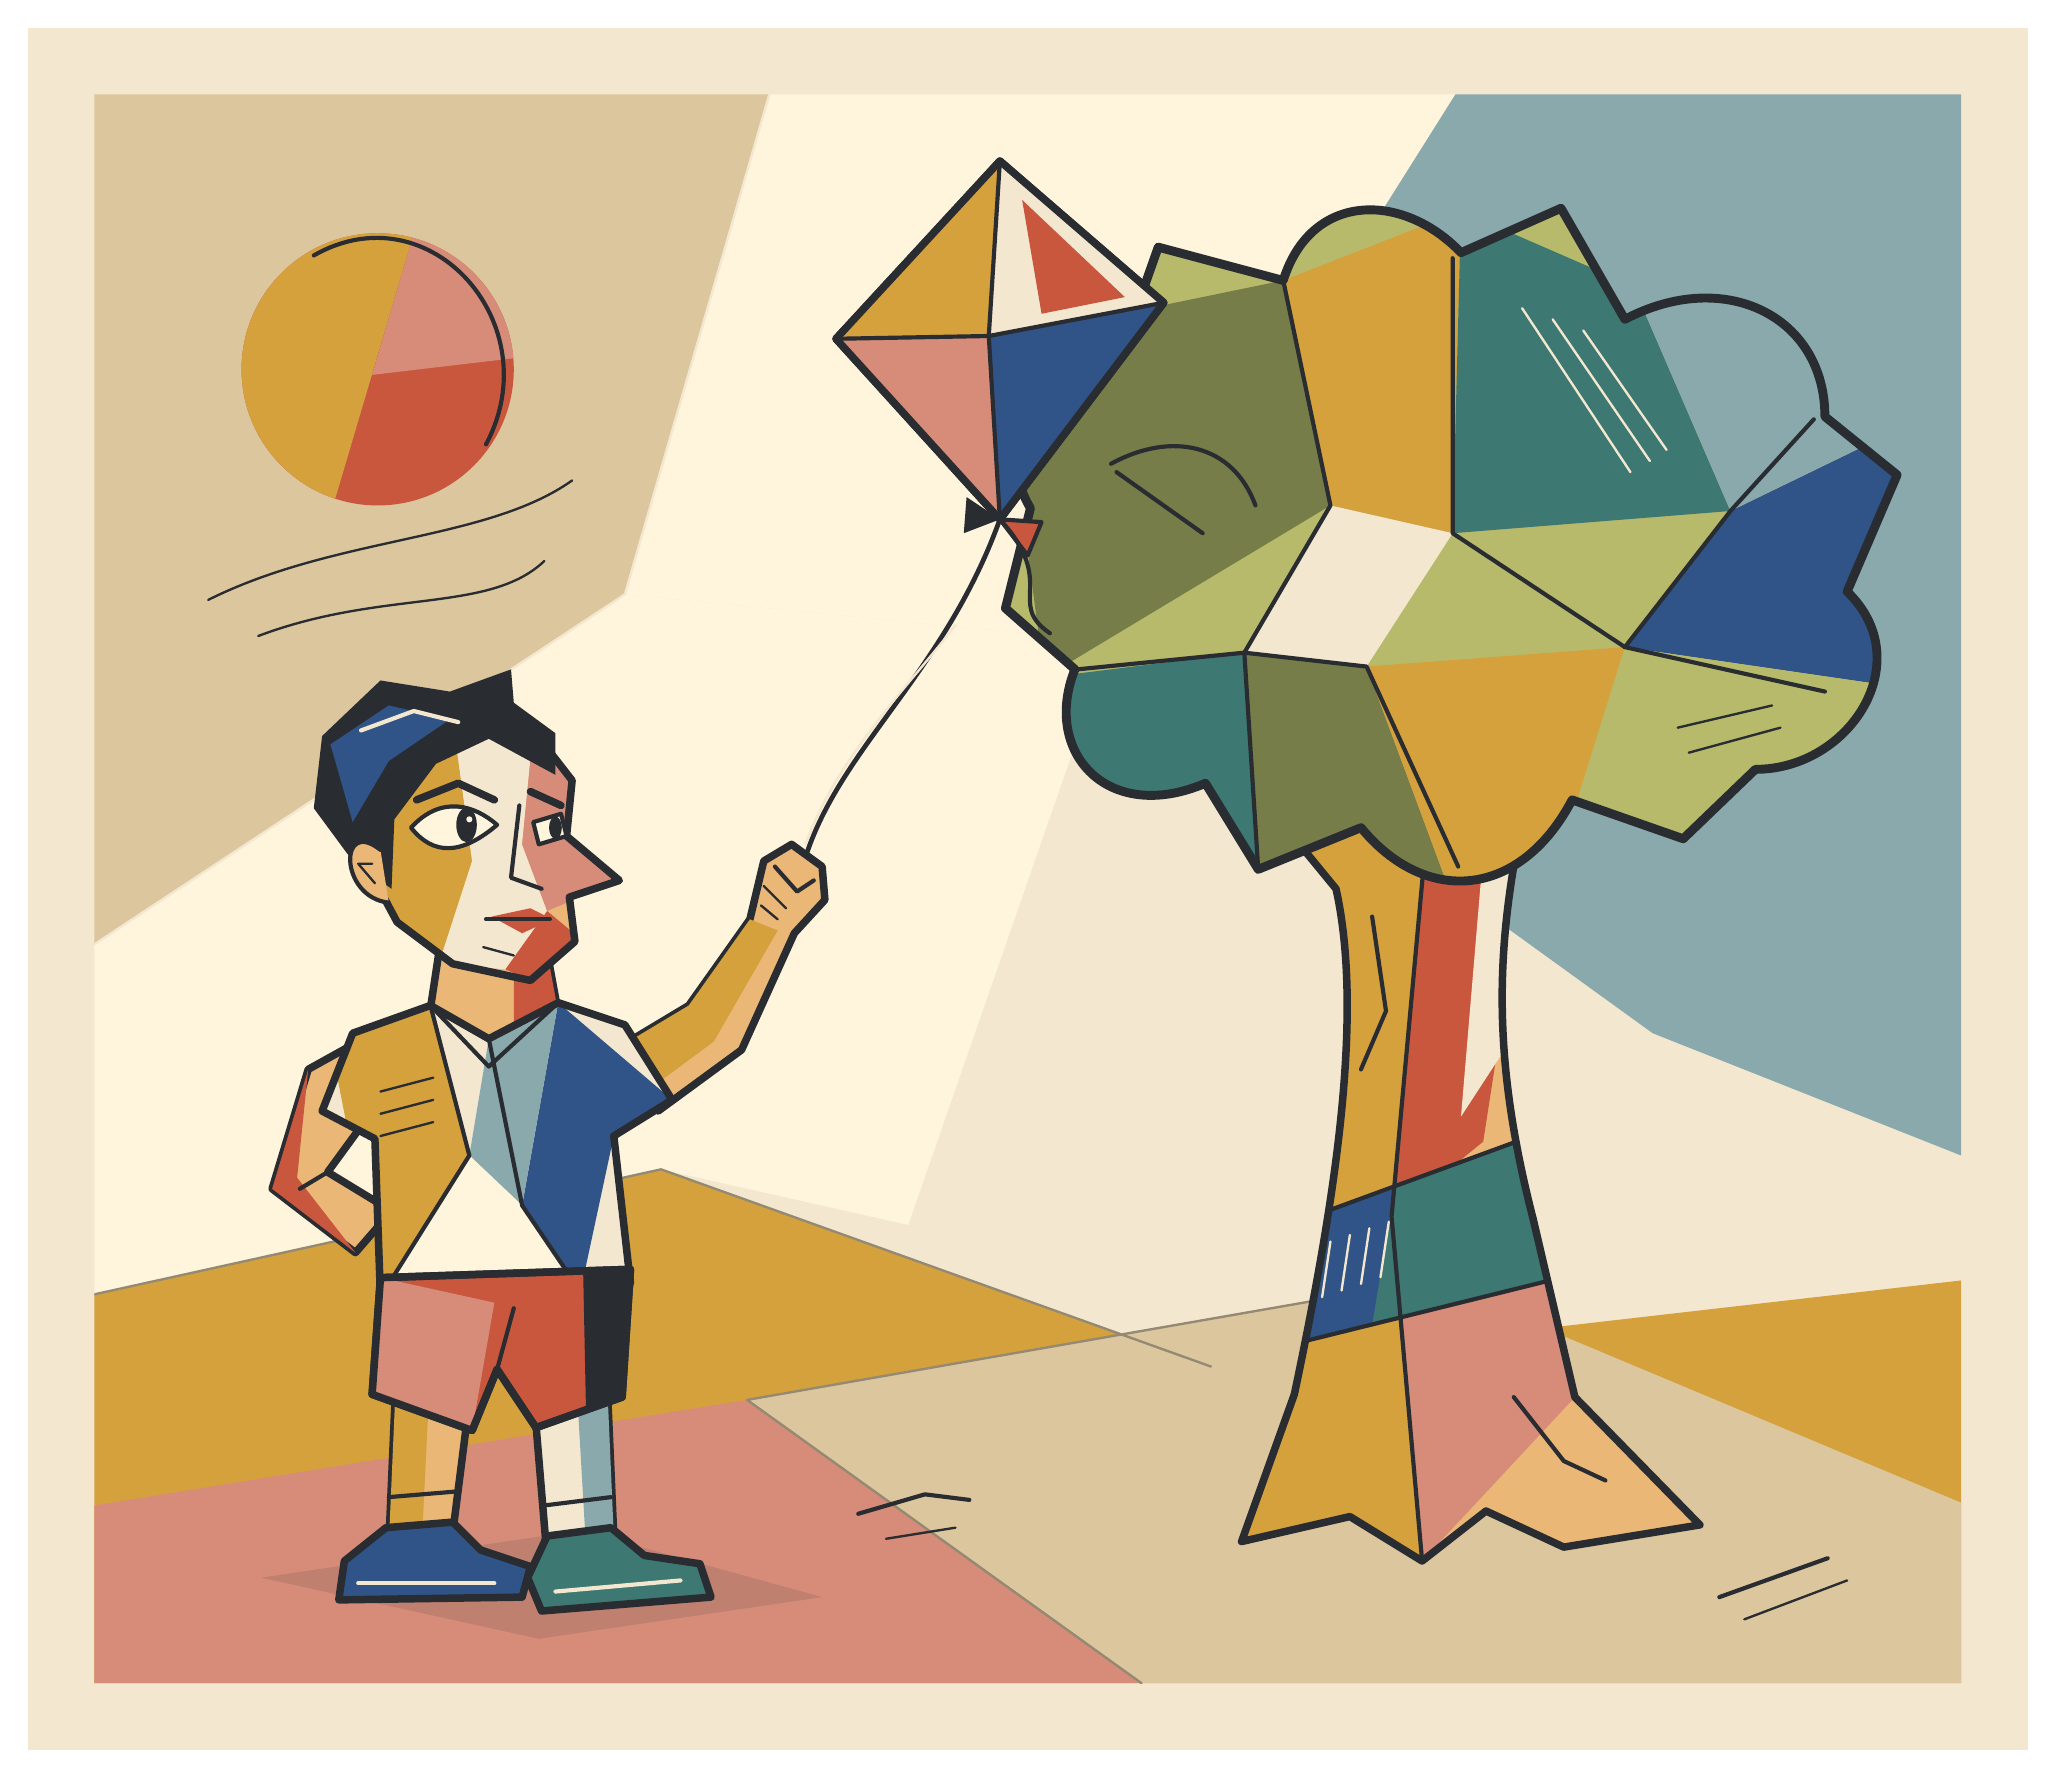
\begin{tikzpicture}[x=1bp,y=-1bp,line cap=round,line join=round,
  contour/.style={draw=ink,line width=2.7bp},
  detail/.style={draw=ink,line width=1.5bp},
  fine/.style={draw=ink,line width=0.85bp}]
  \path[use as bounding box] (0,0) rectangle (720,620);
  \fill[paper] (0,0) rectangle (720,620);
  \begin{scope}
    \clip (24,24) rectangle (696,596);

    % 1. Interlocking planes establish a shallow, deliberately tilted space.
    \fill[sand] (24,24) -- (267,24) -- (215,204) -- (24,330) -- cycle;
    \fill[chalk] (267,24) -- (514,24) -- (390,221) -- (215,204) -- cycle;
    \fill[bluegrey] (514,24) -- (696,24) -- (696,406)
      -- (585,362) -- (390,221) -- cycle;
    \fill[ochre] (24,456) -- (228,411) -- (426,482)
      -- (696,451) -- (696,596) -- (24,596) -- cycle;
    \fill[rose] (24,532) -- (259,494) -- (401,596) -- (24,596) -- cycle;
    \fill[sand] (259,494) -- (505,451) -- (696,531) -- (696,596)
      -- (401,596) -- cycle;
    \fill[chalk] (24,330) -- (215,204) -- (390,221)
      -- (317,431) -- (228,411) -- (24,456) -- cycle;
    \draw[fine,draw=paper] (267,24) -- (215,204) -- (24,330);
    \draw[fine,draw=ink!40!sand] (24,456) -- (228,411) -- (426,482);
    \draw[fine,draw=ink!40!sand] (401,596) -- (259,494) -- (505,451);

    % A split sun balances the tree's visual mass without competing with it.
    \fill[vermilion] (126,123) circle[radius=49bp];
    \begin{scope}
      \clip (126,123) circle[radius=49bp];
      \fill[ochre] (77,74) -- (139,74) -- (110,172) -- (77,172) -- cycle;
      \fill[rose] (139,74) -- (175,74) -- (175,119) -- (124,125) -- cycle;
    \end{scope}
    \draw[detail] (103,82) .. controls (145,58) and (188,107) .. (165,150);
    \draw[fine] (65,206) .. controls (111,183) and (165,185) .. (196,163);
    \draw[fine] (83,219) .. controls (128,202) and (166,211) .. (186,192);

    % 2. Tree: one silhouette clips all trunk planes, avoiding doubled edges.
    \def\Trunk{(471,257) -- (505,275) -- (548,246)
      .. controls (529,314) and (524,359) .. (542,429)
      -- (557,493) -- (602,539) -- (553,547) -- (525,534)
      -- (502,552) -- (476,536) -- (437,545) -- (456,492)
      .. controls (471,421) and (481,355) .. (471,310)
      -- (448,282) -- cycle}
    \path[fill=apricot] \Trunk;
    \begin{scope}
      \clip \Trunk;
      \fill[ochre] (450,245) -- (505,275) -- (502,552) -- (432,552) -- cycle;
      \fill[vermilion] (505,275) -- (548,246) -- (524,401) -- (491,428) -- cycle;
      \fill[paper] (524,297) -- (538,276) -- (531,369) -- (516,392) -- cycle;
      \fill[rose] (491,428) -- (542,411) -- (557,493) -- (502,552) -- cycle;
      \fill[teal] (446,434) -- (536,401) -- (548,451) -- (447,476) -- cycle;
      \fill[cobalt] (446,434) -- (492,418) -- (484,467) -- (447,476) -- cycle;
      \draw[detail] (505,275) -- (491,428) -- (502,552);
      \draw[detail] (446,434) -- (536,401);
      \draw[detail] (447,476) -- (548,451);
      \foreach \x in {0,7,14,21}
        \draw[fine,draw=paper] (469+\x,437-0.34*\x) -- (466+\x,457-0.34*\x);
    \end{scope}
    \draw[contour] \Trunk;
    \draw[detail] (484,320) -- (489,354) -- (480,375);
    \draw[detail] (535,493) -- (553,516) -- (568,523);

    % Crown: a curved outer rhythm, large angular interior planes, sparse veins.
    \def\Crown{(361,173)
      .. controls (346,148) and (364,116) .. (395,113)
      -- (407,79) -- (452,91)
      .. controls (462,59) and (495,59) .. (516,81)
      -- (552,65) -- (575,105)
      .. controls (611,86) and (647,104) .. (647,140)
      -- (673,161) -- (655,203)
      .. controls (681,228) and (656,267) .. (622,267)
      -- (596,292) -- (556,278)
      .. controls (537,314) and (503,316) .. (480,288)
      -- (443,303) -- (424,272)
      .. controls (389,287) and (365,261) .. (377,231)
      -- (352,209) -- cycle}
    \path[fill=citron] \Crown;
    \begin{scope}
      \clip \Crown;
      \fill[olive] (350,112) -- (452,91) -- (469,172) -- (366,234) -- cycle;
      \fill[ochre] (452,91) -- (516,66) -- (513,182) -- (469,172) -- cycle;
      \fill[teal] (516,66) -- (578,93) -- (613,174) -- (513,182) -- cycle;
      \fill[cobalt] (613,174) -- (683,140) -- (671,237) -- (575,223) -- cycle;
      \fill[bluegrey] (578,93) -- (663,96) -- (683,140) -- (613,174) -- cycle;
      \fill[paper] (469,172) -- (513,182) -- (482,230) -- (438,225) -- cycle;
      \fill[teal] (366,234) -- (438,225) -- (443,309) -- (360,282) -- cycle;
      \fill[olive] (438,225) -- (482,230) -- (515,319) -- (443,309) -- cycle;
      \fill[ochre] (482,230) -- (575,223) -- (556,284) -- (515,319) -- cycle;
      \fill[citron] (575,223) -- (671,237) -- (622,289) -- (556,284) -- cycle;
      \draw[detail] (452,91) -- (469,172) -- (438,225) -- (443,303);
      \draw[detail] (513,83) -- (513,182) -- (575,223) -- (647,239);
      \draw[detail] (378,231) -- (438,225) -- (482,230) -- (515,302);
      \draw[detail] (575,223) -- (613,174) -- (643,141);
      \draw[fine,draw=paper] (538,101) -- (577,160);
      \draw[fine,draw=paper] (549,105) -- (584,156);
      \draw[fine,draw=paper] (560,109) -- (590,152);
      \draw[detail] (390,157) .. controls (412,145) and (434,150) .. (442,172);
      \draw[detail] (392,160) -- (423,182);
      \draw[fine] (594,252) -- (628,244);
      \draw[fine] (598,261) -- (631,252);
    \end{scope}
    \draw[contour,line width=3.2bp] \Crown;

    % 3. The kite and hand are joined by one uninterrupted, legible string.
    \coordinate (held-string) at (277,311);
    \coordinate (kite-knot) at (350,177);
    \draw[draw=ink,line width=1.7bp] (held-string)
      .. controls (285,264) and (328,238) .. (kite-knot);
    \draw[fine,draw=paper] (280,294)
      .. controls (292,261) and (320,234) .. (334,215);
    \path[fill=vermilion,contour] (350,48) -- (409,99)
      -- (350,177) -- (291,112) -- cycle;
    \fill[ochre] (350,48) -- (346,111) -- (291,112) -- cycle;
    \fill[paper] (350,48) -- (409,99) -- (346,111) -- cycle;
    \fill[cobalt] (346,111) -- (409,99) -- (350,177) -- cycle;
    \fill[rose] (291,112) -- (346,111) -- (350,177) -- cycle;
    \fill[vermilion] (358,62) -- (395,97) -- (365,103) -- cycle;
    \draw[contour] (350,48) -- (409,99) -- (350,177) -- (291,112) -- cycle;
    \draw[detail] (350,48) -- (346,111) -- (350,177);
    \draw[detail] (291,112) -- (346,111) -- (409,99);
    \path[fill=ink] (350,177) -- (338,169) -- (337,182) -- cycle;
    \path[fill=vermilion,detail] (350,177) -- (365,178) -- (360,190) -- cycle;
    \draw[detail] (350,177) .. controls (371,200) and (352,207) .. (368,218);

    % 4. Boy: short proportions, red shorts, dark hair, and raised gripping hand.
    % Flattened shadows ground the feet without imposing a single perspective.
    \fill[ink,opacity=.12] (84,558) -- (199,541) -- (286,565)
      -- (184,580) -- cycle;
    \path[fill=apricot,contour] (133,477) -- (161,479)
      -- (153,542) -- (130,546) -- cycle;
    \fill[ochre] (133,477) -- (145,482) -- (142,543) -- (130,546) -- cycle;
    \path[fill=paper,contour] (181,479) -- (208,474)
      -- (211,543) -- (187,551) -- cycle;
    \fill[bluegrey] (197,478) -- (208,474) -- (211,543) -- (201,547) -- cycle;
    \draw[detail] (130,529) -- (154,527);
    \draw[detail] (186,532) -- (210,529);
    \path[fill=cobalt,contour] (129,540) -- (153,538) -- (163,548)
      -- (181,554) -- (178,565) -- (112,566) -- (114,552) -- cycle;
    \path[fill=teal,contour] (187,543) -- (210,540) -- (222,550)
      -- (242,553) -- (246,565) -- (185,570) -- (180,558) -- cycle;
    \draw[detail,draw=paper] (119,560) -- (168,560);
    \draw[detail,draw=paper] (190,563) -- (235,559);

    % Folded left arm; raised right arm terminates exactly at held-string.
    \path[fill=apricot,contour] (119,365) -- (101,375) -- (88,418)
      -- (118,441) -- (131,426) -- (108,412) -- (127,386) -- cycle;
    \fill[vermilion] (101,375) -- (97,414) -- (118,441)
      -- (88,418) -- cycle;
    \draw[detail] (108,412) -- (98,418);
    \path[fill=apricot,contour] (213,367) -- (238,352) -- (260,321)
      -- (265,300) -- (275,294) -- (286,302) -- (287,314)
      -- (276,326) -- (257,368) -- (227,390) -- cycle;
    \fill[ochre] (213,367) -- (238,352) -- (260,321)
      -- (270,325) -- (247,365) -- (224,382) -- cycle;
    \draw[detail] (269,302) -- (277,311) -- (283,307);
    \draw[fine] (265,309) -- (273,317);
    \draw[fine] (264,316) -- (270,321);

    % Neck and shirt: a collage of warm paper and cold blue.
    \path[fill=apricot,contour] (150,320) -- (185,322)
      -- (192,360) -- (166,375) -- (145,353) -- cycle;
    \fill[vermilion] (175,325) -- (185,322) -- (192,360) -- (175,366) -- cycle;
    \def\Shirt{(145,352) -- (166,364) -- (191,351) -- (215,359)
      -- (232,386) -- (211,399) -- (217,452) -- (127,457)
      -- (125,400) -- (106,390) -- (117,362) -- cycle}
    \path[fill=paper] \Shirt;
    \begin{scope}
      \clip \Shirt;
      \fill[ochre] (106,350) -- (145,352) -- (159,406) -- (127,457) -- cycle;
      \fill[cobalt] (191,351) -- (232,386) -- (211,399) -- (199,455)
        -- (178,424) -- cycle;
      \fill[bluegrey] (166,364) -- (191,351) -- (178,424) -- (159,406) -- cycle;
      \fill[chalk] (159,406) -- (178,424) -- (199,455) -- (127,457) -- cycle;
      \draw[detail] (145,352) -- (159,406) -- (127,457);
      \draw[detail] (166,364) -- (178,424) -- (199,455);
      \foreach \y in {383,391,399}
        \draw[fine] (127,\y) -- (146,\y-5);
    \end{scope}
    \draw[contour] \Shirt;
    \draw[detail] (145,352) -- (166,374) -- (191,351);

    % Shorts preserve the red cue of the original boy.
    \path[fill=vermilion,contour] (127,450) -- (217,447)
      -- (214,493) -- (183,504) -- (169,483) -- (160,505)
      -- (124,492) -- cycle;
    \fill[rose] (127,450) -- (168,459) -- (160,505) -- (124,492) -- cycle;
    \fill[ink] (200,449) -- (217,447) -- (214,493) -- (201,498) -- cycle;
    \draw[contour] (127,450) -- (217,447) -- (214,493)
      -- (183,504) -- (169,483) -- (160,505) -- (124,492) -- cycle;
    \draw[detail] (169,483) -- (175,461);

    % Face: a frontal almond eye and a displaced profile share one head.
    \def\Face{(120,264) -- (149,244) -- (182,253) -- (196,271)
      -- (194,291) -- (213,307) -- (195,313) -- (197,329)
      -- (181,343) -- (153,337) -- (133,322) -- (118,294) -- cycle}
    \path[fill=apricot] \Face;
    \begin{scope}
      \clip \Face;
      \fill[ochre] (116,254) -- (153,249) -- (160,300) -- (148,337)
        -- (116,321) -- cycle;
      \fill[paper] (153,249) -- (182,253) -- (178,294) -- (187,318)
        -- (172,339) -- (148,337) -- (160,300) -- cycle;
      \fill[rose] (182,253) -- (205,270) -- (194,291) -- (213,307)
        -- (187,318) -- (178,294) -- cycle;
      \fill[vermilion] (172,339) -- (187,318) -- (199,328) -- (181,343) -- cycle;
    \end{scope}
    \draw[contour] \Face;
    \path[fill=ink] (117,300) -- (103,281) -- (106,255)
      -- (127,235) -- (152,239) -- (174,231) -- (175,243)
      -- (190,254) -- (190,269) -- (166,256) -- (147,265)
      -- (132,285) -- (131,310) -- cycle;
    \fill[cobalt] (109,258) -- (130,244) -- (152,249) -- (130,264) -- (117,286) -- cycle;
    \draw[detail,draw=paper] (120,253) -- (139,246) -- (155,250);
    \path[fill=apricot,detail] (127,296)
      .. controls (112,284) and (112,313) .. (130,315);
    \draw[fine] (124,301) -- (119,301) -- (125,308);
    \draw[contour] (140,278) -- (155,272) -- (168,278);
    \path[fill=chalk,detail] (138,288)
      .. controls (149,276) and (161,280) .. (169,287)
      .. controls (156,298) and (146,298) .. (138,288) -- cycle;
    \fill[ink] (158,287) ellipse[x radius=3.7bp,y radius=6.2bp];
    \fill[chalk] (159,285) circle[radius=1.1bp];
    \draw[contour] (181,275) -- (192,280);
    \path[fill=chalk,detail] (182,286) -- (192,283) -- (194,291) -- (184,294) -- cycle;
    \fill[ink] (190,288) ellipse[x radius=2.3bp,y radius=4.0bp];
    \draw[detail] (177,280) -- (174,306) -- (185,310);
    \draw[detail] (194,291) -- (213,307) -- (195,313);
    \path[fill=vermilion] (167,320) -- (181,317) -- (189,321) -- (178,326) -- cycle;
    \draw[detail] (165,321) -- (188,321);
    \draw[fine] (164,331) -- (175,334);

    % A few deliberate ground marks; no labels or simulated artist signature.
    \draw[detail] (299,535) -- (323,528) -- (339,530);
    \draw[fine] (309,544) -- (334,540);
    \draw[detail] (609,565) -- (648,551);
    \draw[fine] (618,573) -- (655,559);
  \end{scope}
\end{tikzpicture}
\end{document}
